
\section{Logo Aplicación}

El logotipo de la aplicación \textbf{Argos} identifica el sistema ante los usuarios. Es minimalista y tecnológico; comunica precisión, enfoque e identificación.

\begin{figure}[h!]
		\centering
		% Se muestra la imagen si existe
		\IfFileExists{./Media/Argos 2.png}{%
			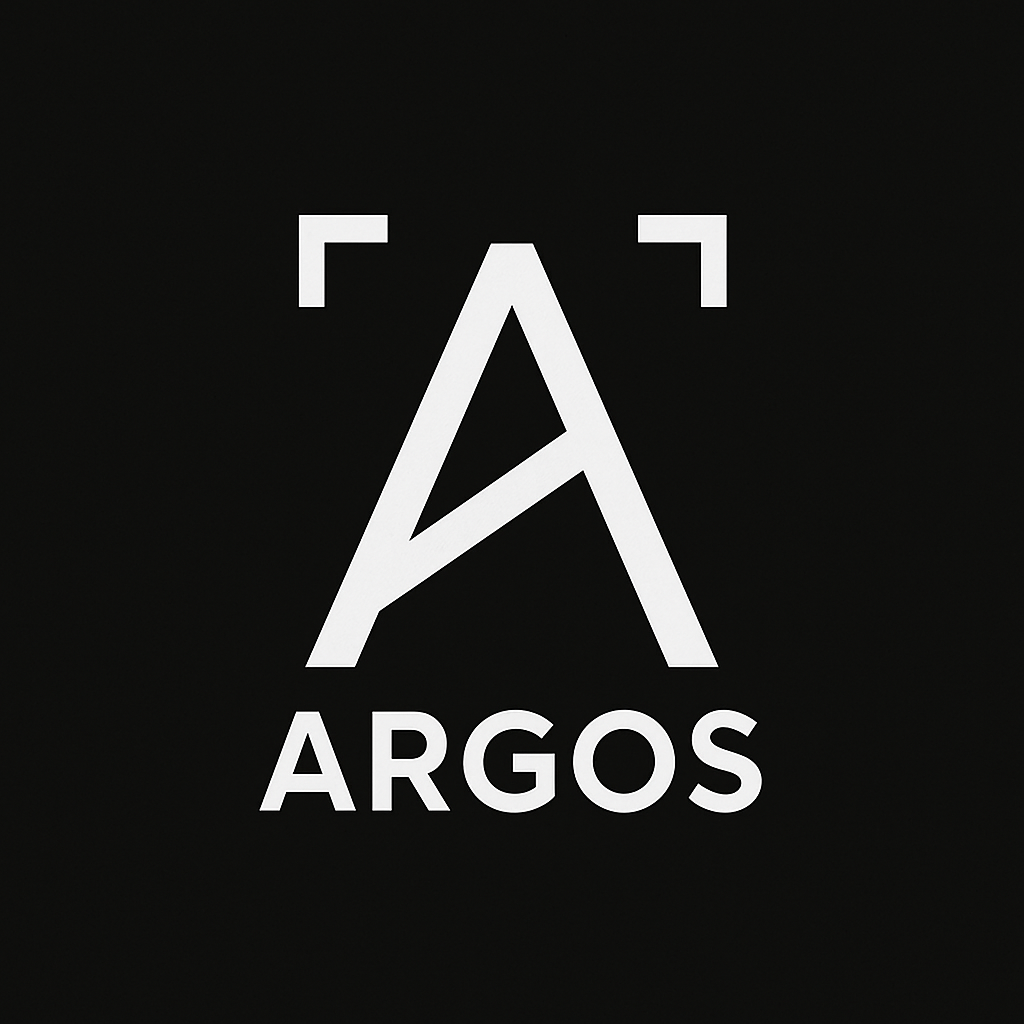
\includegraphics[width=0.3\textwidth]{./Media/Argos 2.png}%
		}{%
			\fbox{\parbox{0.3\textwidth}{\centering Imagen ``Argos 2.jpg'' no disponible}}%
		}
		\caption{Logotipo oficial de la aplicación Argos.}\label{fig:logo_argos}
\end{figure}

\subsection*{Justificación del Diseño}

El concepto refleja la función principal: reconocimiento mediante un marco digital.

\begin{itemize}
		\item \textbf{Elemento central:} Letra “A” mayúscula estilizada que representa “Argos”. Geométrica y limpia; moderna y estable.
		\item \textbf{Marco de enfoque:} La “A” se enmarca con dos corchetes superiores (\texttt{[ ]}) que evocan el marco de una cámara. Comunica escanear, enfocar e identificar.
		\item \textbf{Mensaje general:} Imagen de alta tecnología y precisión; “Argos” como herramienta de identificación.
\end{itemize}

\subsection*{Paleta de Colores}

Paleta monocromática de alto contraste (blanco y negro):

\begin{itemize}
		\item \textbf{Claridad y legibilidad:} Reconocimiento inmediato en cualquier fondo.
		\item \textbf{Modernidad y seriedad:} Estética funcional propia de aplicaciones tecnológicas.
		\item \textbf{Versatilidad:} Se integra con paletas institucionales sin perder identidad.
\end{itemize}

\subsection*{Tipografía}

“ARGOS” usa tipografía \textbf{sans-serif geométrica y en mayúsculas}. Robusta y clara; transmite fiabilidad y solidez.

\subsection*{Aplicación como Icono}

El isotipo (la “A” enmarcada) funciona muy bien como icono en móviles y mantiene legibilidad en tamaños pequeños.
